\documentclass[a4paper,11pt]{article}
\usepackage{amsmath,amssymb}
\usepackage[a4paper,left=19mm,right=19mm,top=40mm,bottom=40mm]{geometry}
\usepackage{txfonts}
\usepackage{kotex}
\usepackage{graphicx}
\usepackage{subfigure}
\usepackage{algorithm}
\usepackage{algpseudocode}
\usepackage{fancyvrb}

\begin{document}
\title{자료구조 HW13-AVLtree}
\author{B935394 컴퓨터공학과 장준희}
\maketitle
\newpage
\section{class설계 내용 및 이유}

처음 클래스의 설계는 다음과 같이 생각했었다. 기본 구조는 이진 탐색 트리를 따라가면서, 회전 기능정도만 추가하고자 했다.
\begin{figure}[h]
\begin{center}
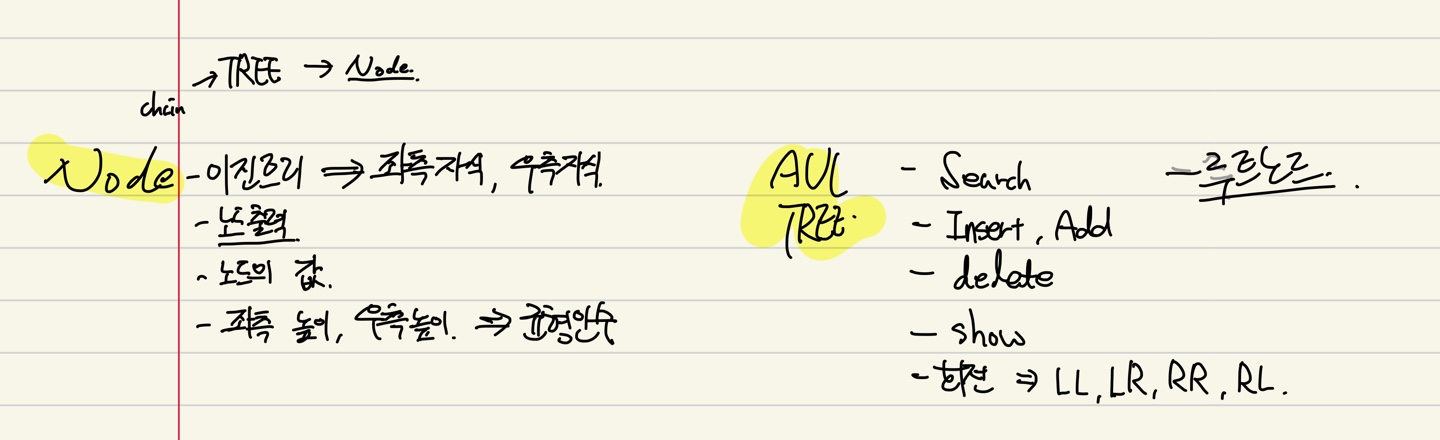
\includegraphics[width=\textwidth]{Struct}
\caption{구조}
\label{fig:fig1}
\end{center}
\end{figure}

최종적인 설계는 다음과 같다.
\subsection{Node Class}
\begin{Verbatim}
class Node{
    friend class AVLtree;
private:
    int value;
    Node * leftChild=nullptr;
    Node * rightChild=nullptr;
    int balFac=0;
    int leftheight=0;
    int rightheight=0;
    int height=0;
    int calHeight(){ return calHeight(this);};
public:
    int calHeight(Node * n);
    int calBF();
    Node(){};
    Node(int a){ value = a; };
    ostream &operator <<(ostream& os){ os<<value; return os; };
};
\end{Verbatim}

삽입, 삭제 과정에서 높이를 단항연산자 등을 이용해 게산하려고 했으나, 막상 회전이나 삭제하는 과정에서 높이를 계산하는게 무리가 있어 트리에서 노드의 높이를 게산하는 함수, 계산된 높이를 토대로 균형인자를 반환해주는 함수가 필요하였다.
\subsection{AVLtree Class}
\begin{Verbatim}
class AVLtree{
private:
    Node * root=nullptr;
public:
    AVLtree(){};
    void Search(int a,Node * n);
    void insert(int a,Node * &n);
    void del(int a, Node * &n);
    void Showresult(Node * n);
    Node* rotate(int key, Node * n);
    void rotateAll(Node *&n);
};
\end{Verbatim}

교재를 보고 틀을 잡아갈 때, 삽입할 때만을 다루고 있어서 재귀적으로 삽입함수를 호출한후, 삽입 함수 말미에 회전 함수를  넣어서 말단 노드부터 회전 연산을 적용할 수 있도록(삽입된 노드에서 가장 가까운 균형 무너진 노드에서 회전 연산이 이루워지도록) 하였다. 그런데, 삭제 함수를 처음 작성할 때, 트리 전체가 흔들린다고 생각하여, 모든 노드를 말단부터 조사하여 필요하다면 회전시켜줄 필요가 있다고 생각했다. 막상 보고서를 작성하면서 다시보니  말미에 회전 연산만 해주었어도 될 것 같다. 

회전 함수의 경우에는 처음에는 반환형을 void로 했었다. 하다보니 노드자체가 바뀌어야한다고 생각해서 Node $*$로 반환형을 바꿔주었다. 삽입과 삭제함수는 인자를 받을 때 참조를 통해받는데, 연산을 할 때에 노드가 변경이 되는 경우가 있어서 그렇게 하였다.
\newpage
\section{결과 값 및 결과 분석}

\begin{figure}[h]
\subfigure[출력]{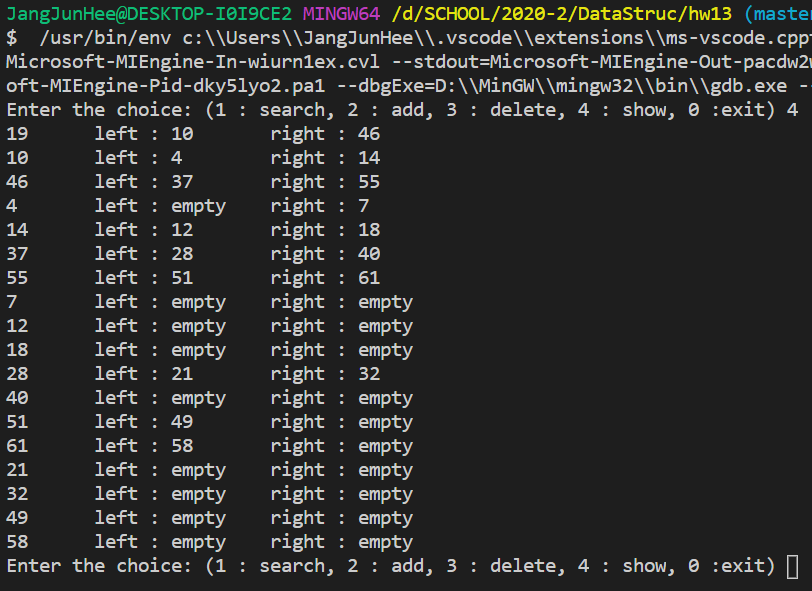
\includegraphics[width=0.3\textwidth]{show}}
\subfigure[삭제/19,18]{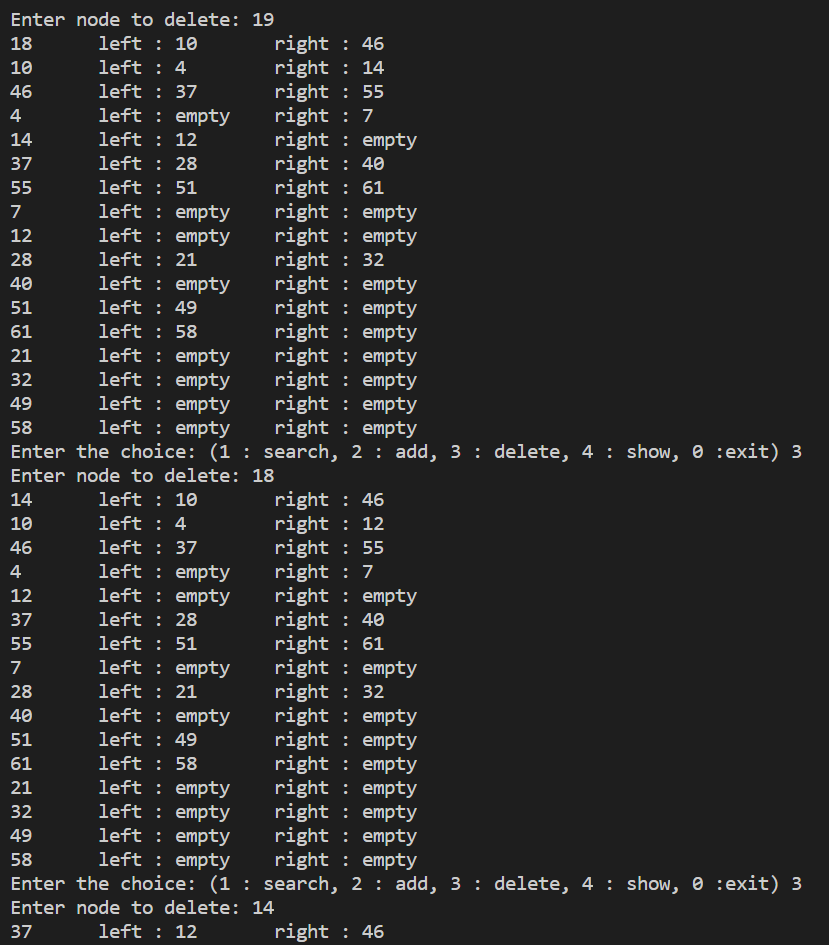
\includegraphics[width=0.3\textwidth]{delete1}}
\subfigure[삭제/14(회전발생)]{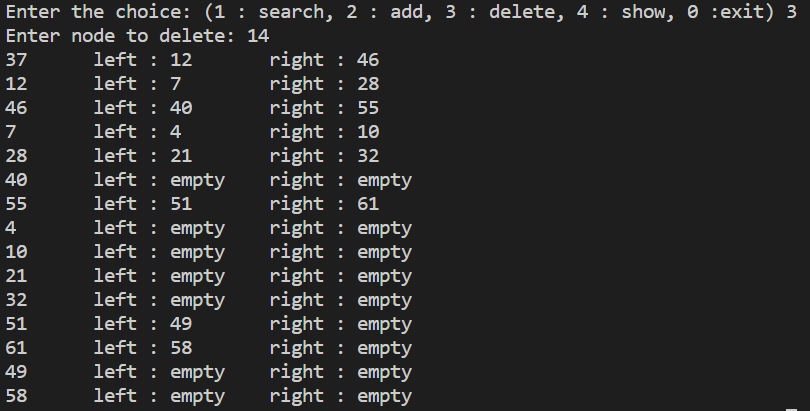
\includegraphics[width=0.3\textwidth]{delete2}}
\caption{출력 및 삭제}
\label{fig:fig2}
\end{figure}
\begin{figure}[h]
\begin{center}
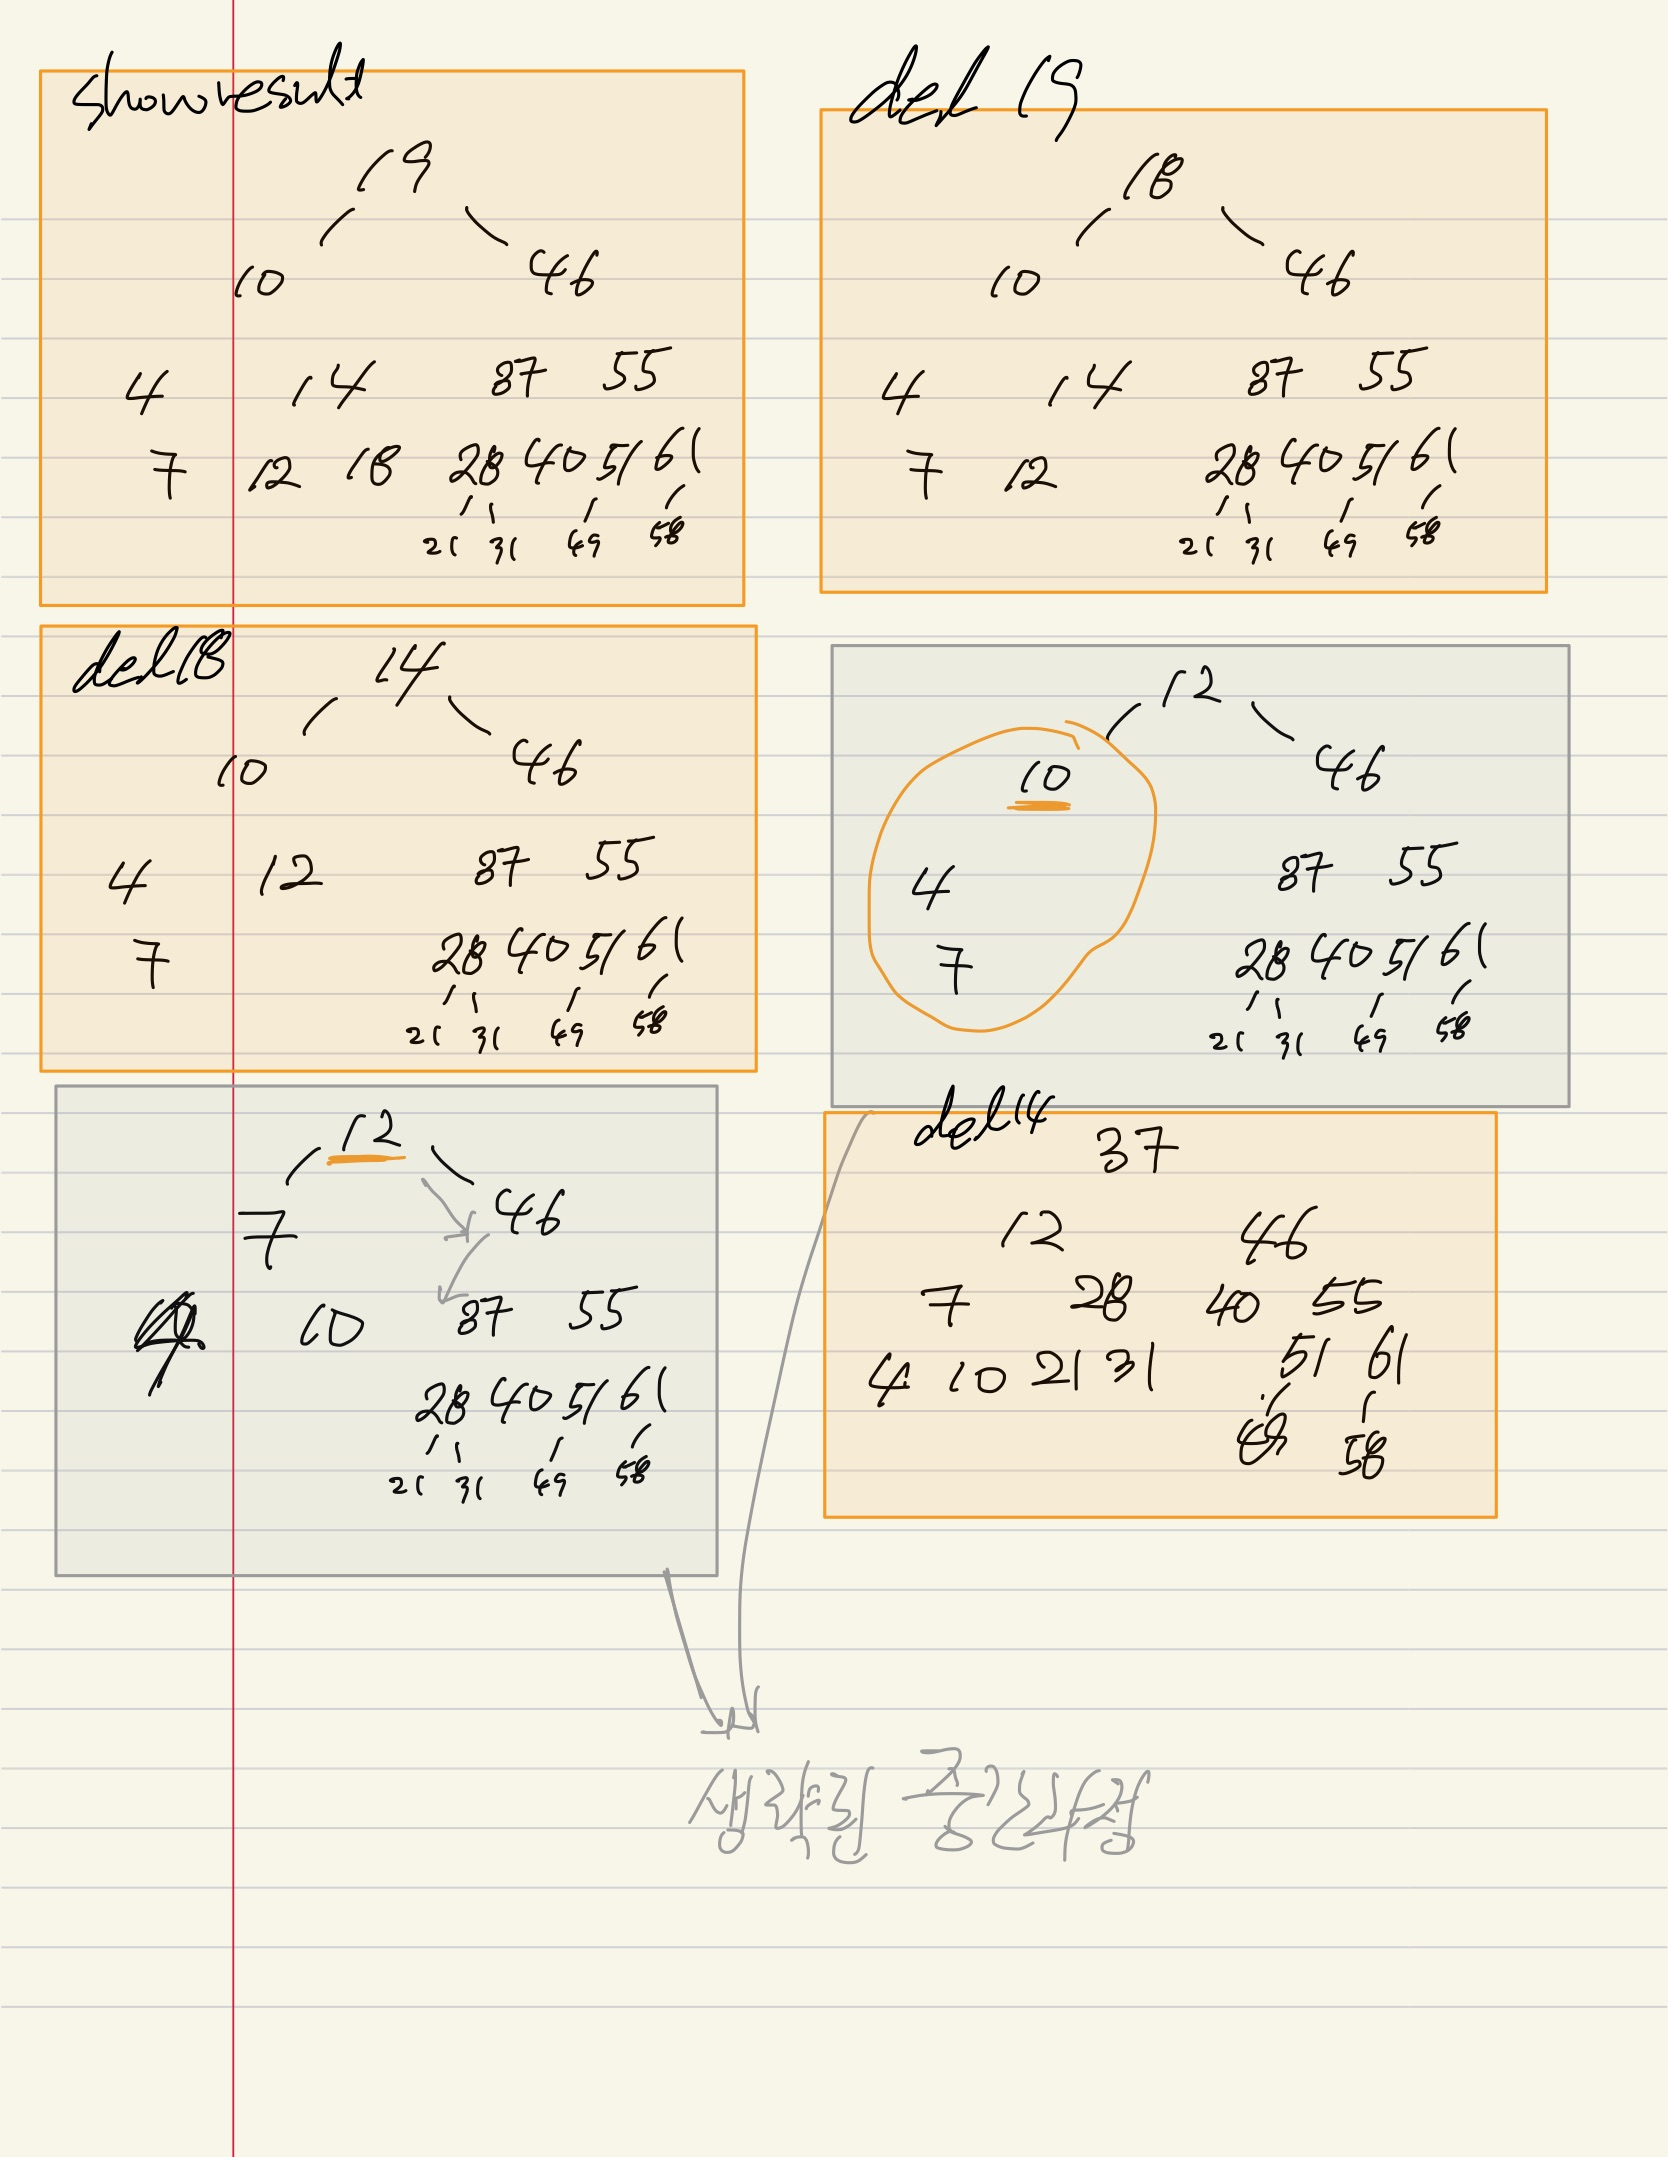
\includegraphics[width=0.3\textwidth]{result}
\caption{분석}
\label{fig:fig3}
\end{center}
\end{figure}

위의 결과출력과 삭제에 대해서 AVLtree가 유지되는 것을 직접 그려가면서 파악할 수 있다.\\\newpage

\begin{figure}[h]
\begin{center}
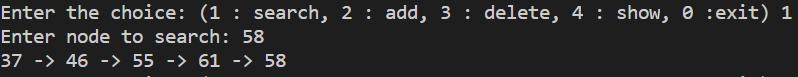
\includegraphics[width=0.6\textwidth]{search}
\caption{탐색}
\label{fig:fig4}
\end{center}
\end{figure}

\begin{figure}[h]
\begin{center}
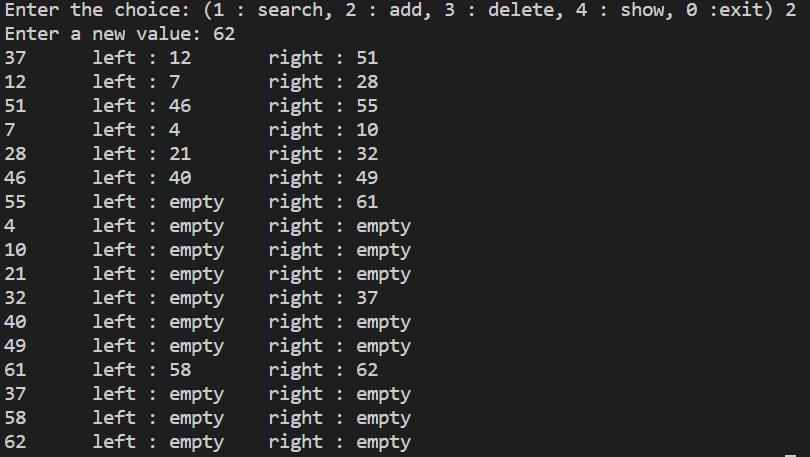
\includegraphics[width=0.6\textwidth]{insert}
\caption{삽입}
\label{fig:fig2}
\end{center}
\end{figure}

위의 삭제연산으로 만들어진 트리에서 탐색과 삽입이 잘 이루워지는 것을 볼 수 있다. 이미 있는 노드의 경우에는 별도의 출력을 하지는않지만, 아무 일도 이뤄지지않는다. 삭제 연산의 경우에는 없는 노드의 경우에 별도의 출력을 하지는 않지만, 아무 일도 이뤄지지 않는다.
\newpage
\section{AVL Tree 연산 설명}
\subsection{회전 연산}
 
\begin{figure}[h]
\begin{center}
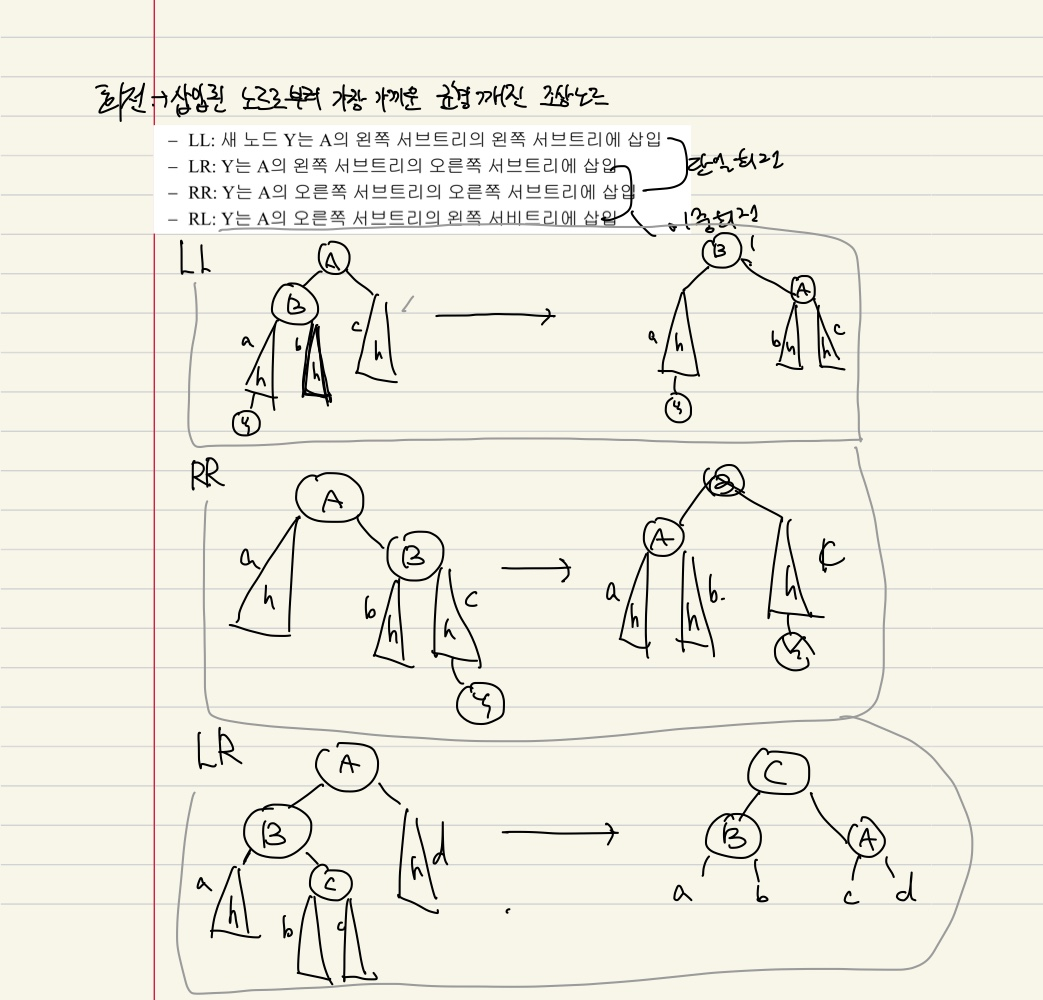
\includegraphics[width=0.6\textwidth]{Rotate}
\caption{회전}
\label{fig:fig2}
\end{center}
\end{figure}

회전 연산의 경우에는 LL,LR,RR,RL연산이 있다. 그림으로 다 그리려했으나 각 연산이 ((LL,RR),(LR,RL))대칭이기도 하고, 공간도 없어서 RL연산은 그리지못했다.

\textbf{LL}연산의 경우 B가 부모노드(A)의 위치로, B의 오른편 서브트리가 A의 왼편 서브트리가 된다. \textbf{LR}연산의 경우 C(손자노드)가 부모노드(A)의 위치로, 손자노드의 왼편 서브트리가 자식노드의 오른편 서브트리로, 오른편 서브트리가 부모노드의 왼편 서브트리가 된다.
\\\\

코드는 다음과 같다.
\begin{Verbatim}
Node* AVLtree::rotate(int key, Node * parent){
    Node * Child;
    if(key<=1&&key>=-1) return parent;
    if(key>1){//LL또는 LR회전
        if(parent->leftChild->balFac==1){//LL회전
            Child=parent->leftChild;
            parent->leftChild=Child->rightChild;
            Child->rightChild=parent;
            return Child;
        }
        else{       //LR회전
            Node * grandChild;
            Child=parent->leftChild;
            grandChild=Child->rightChild;
            Child->rightChild=grandChild->leftChild;
            parent->leftChild=grandChild->rightChild;
            grandChild->leftChild=Child;
            grandChild->rightChild=parent;
            return grandChild;
        }
    }
    if(key<-1){//RR또는 RL회전
        if(parent->rightChild->balFac==-1){ //RR회전
            Child=parent->rightChild;
            parent->rightChild=Child->leftChild;
            Child->leftChild=parent;
            return Child;
        }
        else{       //RL 회전
            Node * grandChild;
            Child=parent->rightChild;
            grandChild=Child->leftChild;
            Child->leftChild=grandChild->rightChild;
            parent->rightChild=grandChild->leftChild;
            grandChild->rightChild=Child;
            grandChild->leftChild=parent;
            return grandChild;
        }
    } 
}
\end{Verbatim}

각 회전을 분리할수도있었겠지만, 분리하는 것보다는 노드와 노드의 균형인자를 넘겨주어 각 회전을 적용하는게 더 간편하다고 생각했다
\subsection{기타 연산}

기타 연산에는 높이구하기, 균형인자구하기, 탐색, 삽입, 삭제, 전수조사해서 회전하기 등이 있다. 탐색, 삽입, 삭제의 경우에는 균형을 잡는 것을 제외하고는 이진 탐색 트리와 동일하다.
\begin{Verbatim}
void AVLtree::Search(int a,Node * n){   //a 찾고자 하는 값, n은 root노드
    Node* curNode;
    curNode=n;
    while(curNode->value!=a){
        cout<<curNode->value<<" -> ";
        if(curNode->value<a)
            curNode=curNode->rightChild;
        else
            curNode=curNode->leftChild;        
    }
    cout<<curNode->value<<endl;
}

void AVLtree::insert(int a,Node * &n){
    Node * curNode=n;
    if(root==nullptr)
        root=new Node(a);
    if(n==NULL){
        curNode=this->root;
        n=curNode;
        return;
    }
    if(a>curNode->value){
        if(curNode->rightChild==nullptr)
            curNode->rightChild=new Node(a);
        else
            insert(a, curNode->rightChild);
    }
    else{
        if(curNode->leftChild==nullptr)
            curNode->leftChild=new Node(a);
        else
            insert(a, curNode->leftChild);
    }
    //재귀함수이므로 리프노드에 제일 가까운 균형무너진 조상에서 회전이 일어남
    n=rotate(n->calBF(), n); 
}

void AVLtree::del(int a, Node * &n){
    Node * curNode=n;
    static Node * parent;
    static bool check=0;
    if(curNode==nullptr) return;
    if(a==curNode->value){ 
        if(curNode==root){      //root노드일때
            if(curNode->rightChild==nullptr&&curNode->leftChild==nullptr){
                delete curNode; curNode=nullptr;
            }
            else if(curNode->rightChild==nullptr||curNode->rightChild==nullptr){
                if(curNode->rightChild==nullptr)
                    root=curNode->leftChild;
                else
                    root=curNode->rightChild;
                delete curNode; curNode=nullptr;
            }
            else{   //작은 것들 중 제일큰 노드->루트노드
                Node * parent2;
                Node * temp=root;
                parent2=curNode;
                curNode=curNode->leftChild;
                while(curNode->rightChild!=nullptr){
                    parent2=curNode;
                    curNode=curNode->rightChild;
                }
                if(curNode->leftChild!=nullptr)
                    parent2->rightChild=curNode->leftChild;
                else
                    parent2->rightChild=nullptr;
                curNode->rightChild=temp->rightChild;
                curNode->leftChild=temp->leftChild;
                root=curNode;
                delete temp;
            }
        
        }
        else{   //root노드 아닐때
            if(curNode->rightChild==nullptr&&curNode->leftChild==nullptr){
                if(check==0){   //parent의 우측 자식
                    parent->rightChild=nullptr;
                }
                else{
                    parent->leftChild=nullptr;
                }
                delete curNode; curNode=nullptr;
            }
            else if(curNode->rightChild==nullptr||curNode->rightChild==nullptr){
                if(check==0)
                    parent->rightChild=curNode->rightChild;
                else
                    parent->leftChild=curNode->leftChild;
                delete curNode; curNode=nullptr;
            }
            else{   //좌측의 가장 큰 노드를 삽입
                Node * parent2;
                parent2=curNode;
                curNode=curNode->leftChild;
                while(curNode->rightChild!=nullptr){
                    parent2=curNode;
                    curNode=curNode->rightChild;
                }
                parent2->rightChild=nullptr;
                if(check==0){
                    curNode->rightChild=parent->rightChild->rightChild; 
                    curNode->leftChild=parent->rightChild->leftChild;
                    delete parent->rightChild;
                    parent->rightChild=curNode;
                }
                else{
                    curNode->rightChild=parent->leftChild->rightChild; 
                    curNode->leftChild=parent->leftChild->leftChild;
                    delete parent->leftChild;
                    parent->leftChild=curNode;
                }
            }
        }
        //삭제하는 과정에서는 트리 전체가 흔들리므로 전수조사필요
        //레벨오더로 읽어서 스택에 저장, 하나씩 조사(제일 가까운 조상노드 때문)
        /*
        queue<Node *> q; stack<Node*> s;
        Node * searchNode=root;
        s.push(searchNode);
        while(searchNode){
            if(searchNode->leftChild!=nullptr){
                q.push(searchNode->leftChild);
            }
            if(searchNode->rightChild!=nullptr){
                q.push(searchNode->rightChild);
            }
            if(q.empty())   break;
            searchNode=q.front(); s.push(q.front()); q.pop(); 
        }
        while(s.empty()==false){
            s.top()=rotate(s.top()->calBF(),s.top());
            s.pop();
        }*/
        rotateAll(root);
        if(parent==nullptr)
            n=this->root;
    }
    else if(a>curNode->value){
        check=0;
        parent=curNode;
        del(a,curNode->rightChild);
    }
    else{
        check=1;
        parent=curNode;
        del(a,curNode->leftChild);
    }
    
}
\end{Verbatim}

삭제함수를 보면, 처음에는 전수조사하여 회전하기를 따로 함수로 빼기 싫어서 큐로 레벨오더로 트리를 읽고, 스택에 저장하여 말단부터 올라가고자 했으나, 트리에 회전이 반영이 안될 때도 있고, 참조도 안되고 하여 따로 함수로 뺐다.
\begin{Verbatim}
int Node::calHeight(Node * n){
    if(n!=nullptr){
        n->leftheight=calHeight(n->leftChild);
        n->rightheight=calHeight(n->rightChild);
        n->height=max(n->leftheight,n->rightheight)+1;
    }
    if(n==nullptr) return 0;
    return n->height;
}

int Node::calBF(){
    this->calHeight();
    balFac=this->leftheight-this->rightheight;
    return balFac;
}

void AVLtree::rotateAll(Node *&n){ 	//재귀를 통해 말단부터 조사
    if(n->rightChild!=nullptr)
        rotateAll(n->rightChild);
    if(n->leftChild!=nullptr)    
        rotateAll(n->leftChild);
    n=rotate(n->calBF(),n);
}
\end{Verbatim}

높이 구하는 함수의 경우에는 노드의 왼편 서브트리의 높이와, 오른편 서브트리 높이 중 더 큰 것에 1을 더한 것으로 삼았다. 균형인자는 왼편 서브트리 높이와 오른편 서브트리의 차로 구하였다. 전수조사하여 회전하기 는 재귀호출을 통해 말단부터 조사가 되도록 하였다.

트리를 출력하는 함수는 이진탐색트리의 레벨오더로 읽는 것을 활용하였다.

\end{document}